Here we provide the background for the \nameTurbulence\ project (Section
\ref{subsec.turb_motivate})
and briefly motivate the simulations to support this study (Section
\ref{subsec.turb_sims})  Details of the
simulation cost can be found in Section \ref{subsec.turb_accounting}.


\subsubsection{Motivation}
\label{subsec.turb_motivate}

The interstellar medium (ISM) is the gas between stars in the galaxy.  It cools
very effectively, so can be treated as isothermal \red{Krumholz star formation
book}.  The ISM is also turbulent, with supersonic shocks driven by supernovae
causing supersonic turbulence throughout the interstellar medium.  This
turbulence impacts the formation of stars (see Section \ref{sec.back_cores}) and
causes a polarized screen that is blocking our view of the light from the big bang (see
Section \ref{sec.back_foregrounds}), among many other effects
\citep{Elmegreen04}. It is also interesting in its own right.

Supersonic turbulence is compressible, and the distribution of density
fluctuations is described by a log normal, i.e. the log of density is
distributed as a gaussian.  The distribution of velocity is roughly Maxwellian,
i.e. each of the components is a guassian, and added in quadrature the
distribution is Maxwellian.  
We have recently found analytic distributions for the internal energy and
kinetic energy, as well as their joint
distribution.   These energy distributions will be useful
in future studies of turbulence in the ISM.  We have verified these formulae 
with lower resolution simulations, with excellent but low-resolution agreement.
Now we wish to verify the formulae with higher resolution simulations, and to
explore if the small deviations from lognormal density and Maxwellian velocity
that were seen in our preliminary runs are numerical, or something more
interersting such as non-local transfer in the turbulent cascade.

Our analytic formulae predict, and the simulations reproduce, interesting
changes in internal energy as the Mach, \mach, number is increased.
The Mach number, \mach, is the r.m.s velocity relative to the speed
of sound, and it dictates how compressible the flow is.  We find that as \mach\
is increases, a step forms at $E_T = 0$, which is reproduced by simulations.


We will perform a series of simulations increasing the r.m.s. 
\begin{figure} \begin{center}
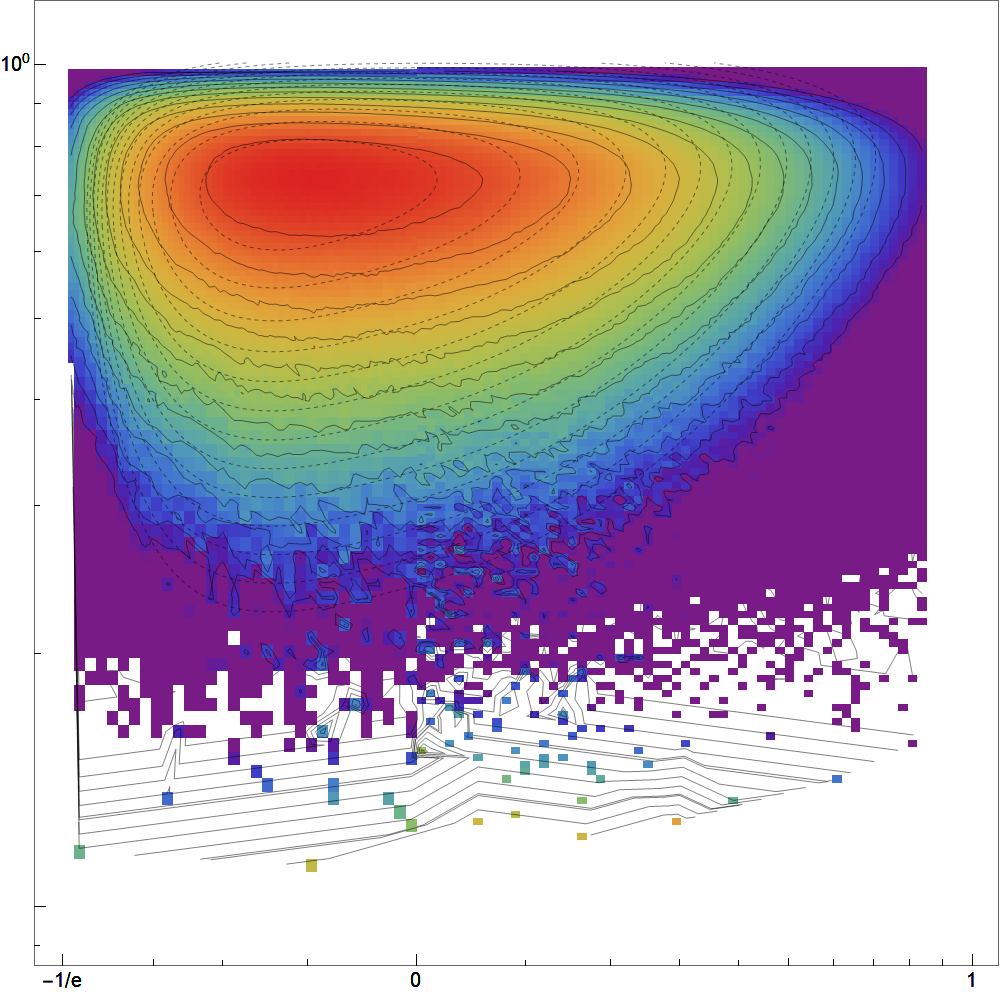
\includegraphics[width=0.32\textwidth]{figs/mach5_contours_comparison_V_MCMC.png}
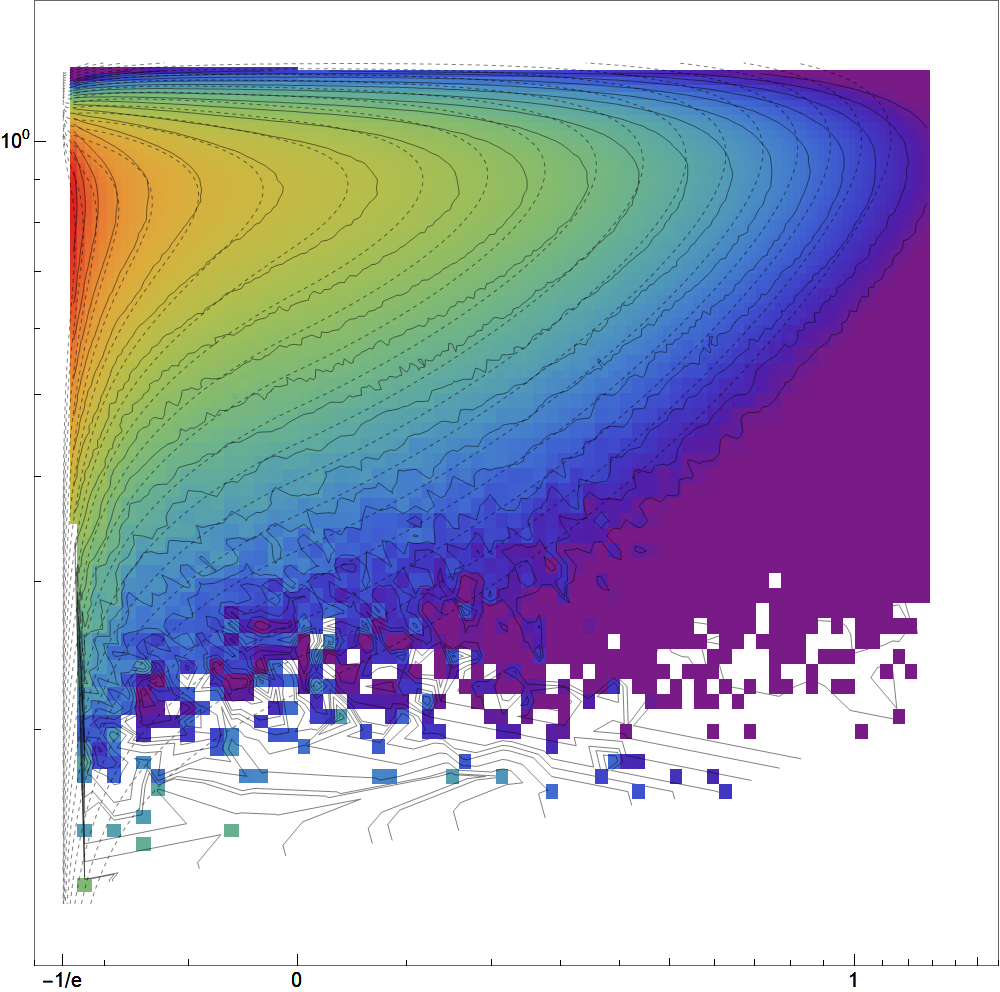
\includegraphics[width=0.32\textwidth]{figs/mach10_contours_comparison_V_MCMC.png}
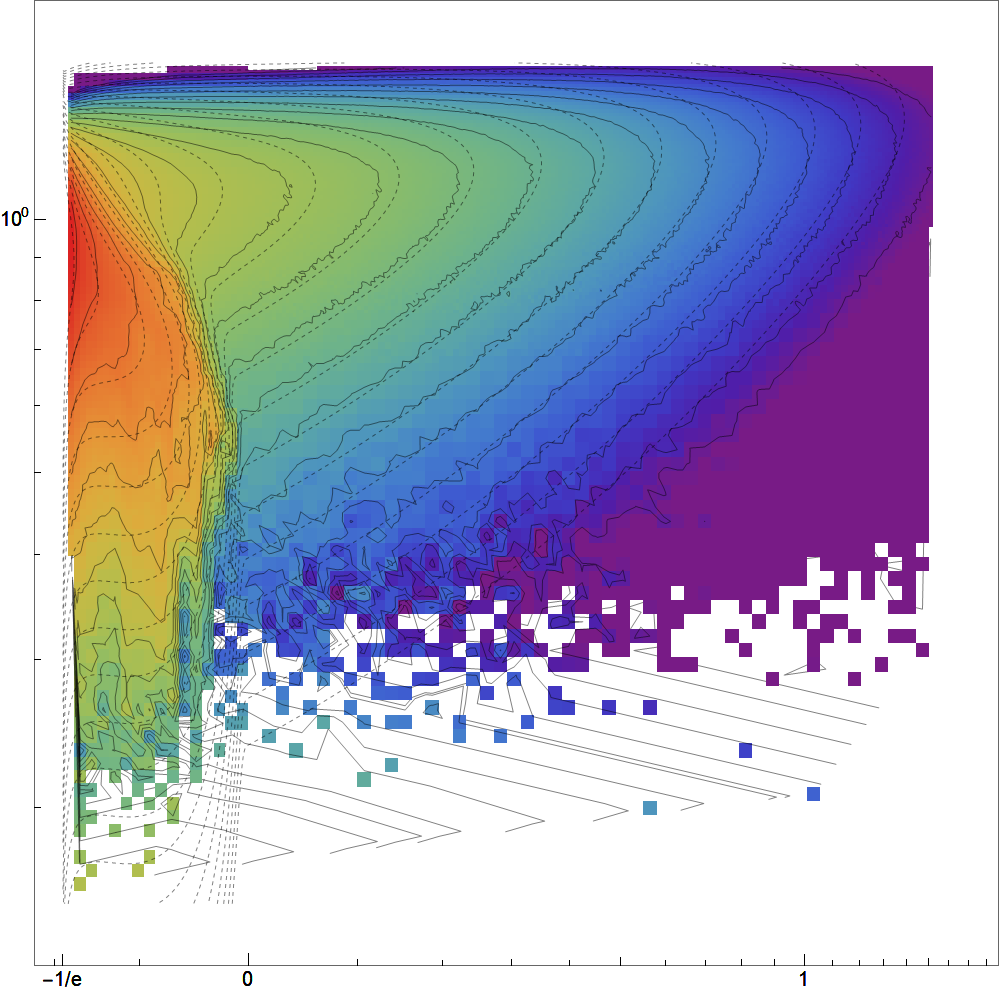
\includegraphics[width=0.32\textwidth]{figs/mach20_contours_comparison_V_MCMC.png}
\caption[ ]{The joint distribution between thermal energy, $E_T$, and kinetic
energy $E_K$. Color shows the PDF computed from low resolution simulations, and ranges between 0 (purple) and 1
(red).  The thermal energy develops a low $E_T$ wall as well as a high $E_T$
wing as the Mach number increases.  We will improve the noise and accuracy of
these fits.}
\label{} \end{center} \end{figure}

\subsubsection{Simulations}
\label{subsec.turb_sims}

Our simulations will begin with uniform density, and \red{magic paddles}

\red{We will perform $1024^3$  simulations because it should be a lot better}
